% úvod o kapitole, přehled

\section{Strand models}
	
	There exist (can be synthesized) many types of molecules, well described by Winfree \cite{winfree_phd} even with their inception reaction. These can form linear strands (sections \ref{sec:adleman}, \ref{sec:lin_strands}), dendrimer structures (section \ref{sec:dendri}) or 2D tilings (section \ref{sec:double_cross}).
	
	\subsection{Adleman's experiment}
	\label{sec:adleman}
		
		Adleman showed in his ground-breaking work \cite{adleman94} that DNA molecules are really capable of computation. He exploited that huge parallelism possible in DNA computation for one of the most fundamental $\NP$-complete problems -- the Hamiltonian Path Problem (HPP) in directed graph with designated vertices $v_{begin}$ and $v_{end}$.
		
		Let us remind this type of HPP. Given a directed graph $G_n$ with $n$ vertices and two designated vertices $v_{begin}$ and $v_{end}$, the problem is to answer whether there exists an oriented path from $v_{begin}$ to $v_{end}$ through the graph such that the path visits every vertex. Note that {\em path} cannot visit any vertex more than once from definition.
		
		\begin{figure}[H]
		\begin{center}
			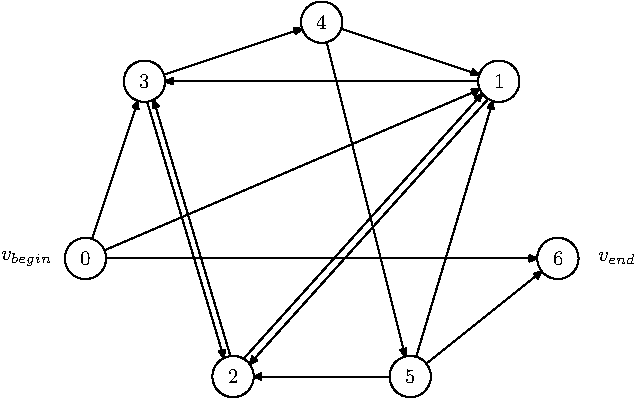
\includegraphics{./figures/adleman_graph.pdf}
			\caption{Adleman's original graph.}
			\label{fig:adleman_graph}
		\end{center}
		\end{figure}
		
		Adleman originally used a graph with seven vertices shown in figure \ref{fig:adleman_graph}. It can be seen that the path $0 \rightarrow 1 \rightarrow 2 \rightarrow 3 \rightarrow 4 \rightarrow 5 \rightarrow 6$ is Hamiltonian\footnote{Note that it can be re-labelled such a nice way without loss of generality.}.
		
		Adleman first presents this non-deterministic five-step algorithm, whose steps are then described in terms of DNA manipulations:
		\begin{description}
			\item[Step 1] Generate random paths through the graph.
			\item[Step 2] Keep only those paths that begin with $v_{begin}$ and end with $v_{end}$.
			\item[Step 3] If the graph has $n$ vertices, then keep only those paths that enter exactly $n$ vertices.
			\item[Step 4] Keep only those paths that enter all of the vertices of the graph at least once.
			\item[Step 5] If any paths remain, say ``Yes''; otherwise, say ``No.''\footnote{This is the original version, I would rectify the fifth step: If any paths remain, say ``Yes''; otherwise say ``{\em I do not know}''. That is because it may happen that there exists a valid path but unfortunately it did not assemble or got lost. Note the similarity to $\NP$ versus $\coNP$, see section \ref{sec:PNP}.} %!% citaci, někdo to už taky kritizoval
		\end{description}
		To see % sloveso od insight ?
		how DNA can compute, let us describe this example more precisely. The computation itself (meaning the inception of the final solution) is hidden in Step 1. Each vertex $i$ is associated with a random\footnote{We will expect those sequences to be different enough.} $20$-mer sequence of DNA, let us denote its $5'\rightarrow 3'$ orientation by $O_i$, its 10-mer prefix by $p_i$ and its 10-mer suffix by $q_i$. Each edge $i\rightarrow j$ is then associated with $\overline{q_i p_j}$ sequence with reverse backbone orientation ($3'\rightarrow 5'$) where $\overline{q_i}$ stands for Watson-Crick complementary word. There is an exception for $i=begin$ and $j=end$: instead of $\overline{q_{begin} p_j}$ there is $\overline{O_{begin} p_j}$ and in a similar way for $j=end$.
		
		\begin{figure}[H]
		\begin{center}
			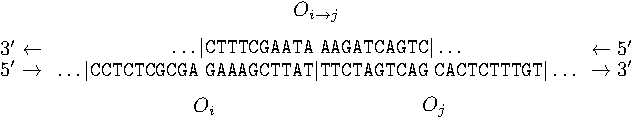
\includegraphics{./figures/adleman_strands.pdf}
			\caption{Example of assigned sequences.}
			\label{fig:adleman_strands}
		\end{center}
		\end{figure}
		
		It can be easily seen that all correctly bonded double-strands correspond with a valid walk through $G_n$. Moreover, all complete double-strands represent a valid walk from $v_{begin}$ to $v_{end}$ through $G_n$.
		
		All the other steps are fully described in \cite{adleman94}. The most important thing is that the most time-demanding step is Step 4. In this step one has to purify the product of Step 3 with a {\em biotin-avidin magnetic beads system}. This process extracts consequently for every vertex $i$ only those DNA strands which contain a substring representing vertex $i$. Thus this algorithm has biostep complexity $O(n)$ which we considered unfeasible. Better solution with biostep complexity $O(1)$ was brought by Winfree \cite{winfree_phd}, see section \ref{sec:double_cross}.
	
	%~ \subsection{Single-stranded molecules}
		%~ 
		%~ As we noted before, the only feasible methods are those computing in $O(1)$ biosteps.
		%~ 
		%~ SAT in $O(1)$ biosteps etc.
	
	%~ \subsection{Double-stranded molecules}
	
	\subsection{Linear strands}
	\label{sec:lin_strands}
		
		Equivalent to regular languages.
	
	\subsection{Dendrimer structures}
	\label{sec:dendri}
		
		Equivalent to context-free languages.
	
	\subsection{Double crossover molecules}
	\label{sec:double_cross}
		
		DAO vs. DAE units. Winfree pg 36 -- sizes of DAE and a better picture, pg 37 -- comparison of DAO/DAE in a lattice, explanation pg 43.
		
		Seeman, Fu and their DAO/DAE in \cite{seeman93}, is the picture of DAO strange?
		
		Equivalent to recursively enumerable languages (Turing universal). Important notes in 3.2.5 Winfree -- single side hybridization -- how to avoid. Tricky solution of Hamiltonian Path Problem.